
\section{Recurrent Neural Networks}

\subsection{Introduction}

Recurrent neural networks (RNN) are a class of neural networks where the connections in the graph can form directed cycles.
This is basically similar to existing neuronal structures like biological brains. 
The cyclic nature of the RNN-graph allows the net to "remember" previous inputs over amounts of time, 
as opposed to other classes of neural networks which are directed acyclic graphs (also called "feed forward")\\

This has the advantage that the RNN can act based on previous events, without having to receive all the context as input at the same time.
A simple example of an RNN can be seen in figure \ref{fig:RNN-rolled}, 
where the net processes the input value $x_t$ and outputs the value $h_t$.
The loop works essentially like copies of the same neural net chained up behind each other and passing it's current
output value $h_{t-1}$ to it's successor: $h_t = \sigma(W_{x} * x_t + W_{h} * h_{t-1})$ 
(Where $W_x$, $W_h$ are the parameters of the gate \textbf{A}).

Following this idea the RNN can be "unrolled" to show the processing of different inputs $x_i$ over time. An example of this can be seen in
the figure \ref{fig:RNN-unrolled}. This way an RNN looks just like a feed forward neural net. This way of looking at recurrent connections
will come up in the section~\ref{subsec:BPTT} where we discuss the training of RNN's.

\begin{wrapfigure}{r}{0.3\textwidth}
  \begin{center}
    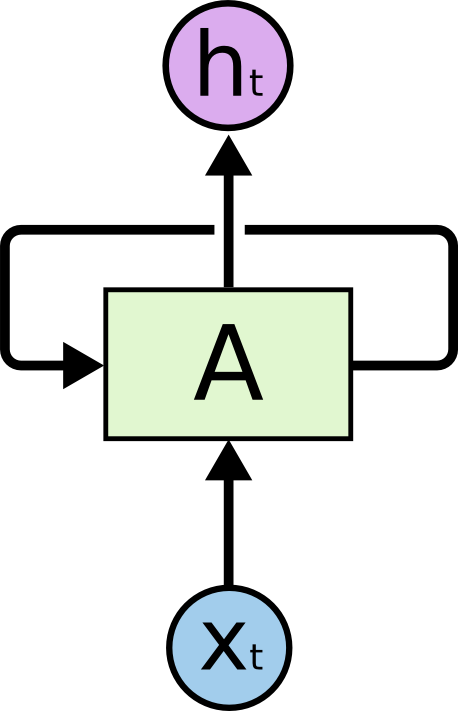
\includegraphics[width=0.4\textwidth]{./img/RNN-rolled}
  \end{center}
  \caption{A basic Recurrent Neural Networks, taking in the value $x_i$ and outputs the value $h_i$ (taken from~\cite{olah:lstm:2015})}
    \label{fig:RNN-rolled}
\end{wrapfigure}

\subsection{Training a RNN: Backpropagation Through Time}
\label{subsec:BPTT}

A common way to train neural networks is the so called "backpropagation of errors". It is a supervised learning method,
this requires having a known desired output value $y_t$ for every training input $x_t$. 
The measure of the difference between the desired and the 
actual output value of the net is the current error $E$, for example $E = \frac{1}{2} (h_t - y_t)^2$. 
The goal with backpropagation is to minimize the error $E$.

In other words we want to set every weight $w_{ij}$ of the neural net such that $E$ becomes minimal, 
the variable $w_{ij}$ denotes the weight for a connection between neurons i and j.
To minimize the error we can use the optimization method of "gradient descent". 
We calculate the gradient of $E$ with regards to the weights of the neural net: $\frac{\partial E}{\partial w_{ij}}$ and
then adjust every weight proportionally to the gradient:
\[
  \Delta w_{ij} = - \alpha \frac{\partial E}{\partial w_{ij}}
\]
In this formula $\alpha$ is a factor to control the speed of the learning process and prevent overfitting\\

We can't just apply backpropagation to an RNN, because this doesn't account for the recursive nature of some of the links. 
A simple solution to this is the method of Backpropagation Through Time (BPTT). As previously described, the recursive 
link in the RNN can be "unrolled" such that the network becomes a normal feed forward network, see figure \ref{fig:RNN-unrolled}. 
The RNN loop is unrolled $t$ times and now contains $t$ instances of $A$ with $t$ inputs. 
If we have some sample data each training pattern consists of
$\langle\mathbf{x}_0,\mathbf{y}_0,\mathbf{x}_{1},\mathbf{x}_{2},\dots,\mathbf{x}_{t},\mathbf{y}_{t}\rangle$, 
where ${y_0,\dots,y_t}$ are the desired outputs.
This sample can then be used for the training with backpropagation and gradient descend.

\begin{figure}[H]
\begin{center}
  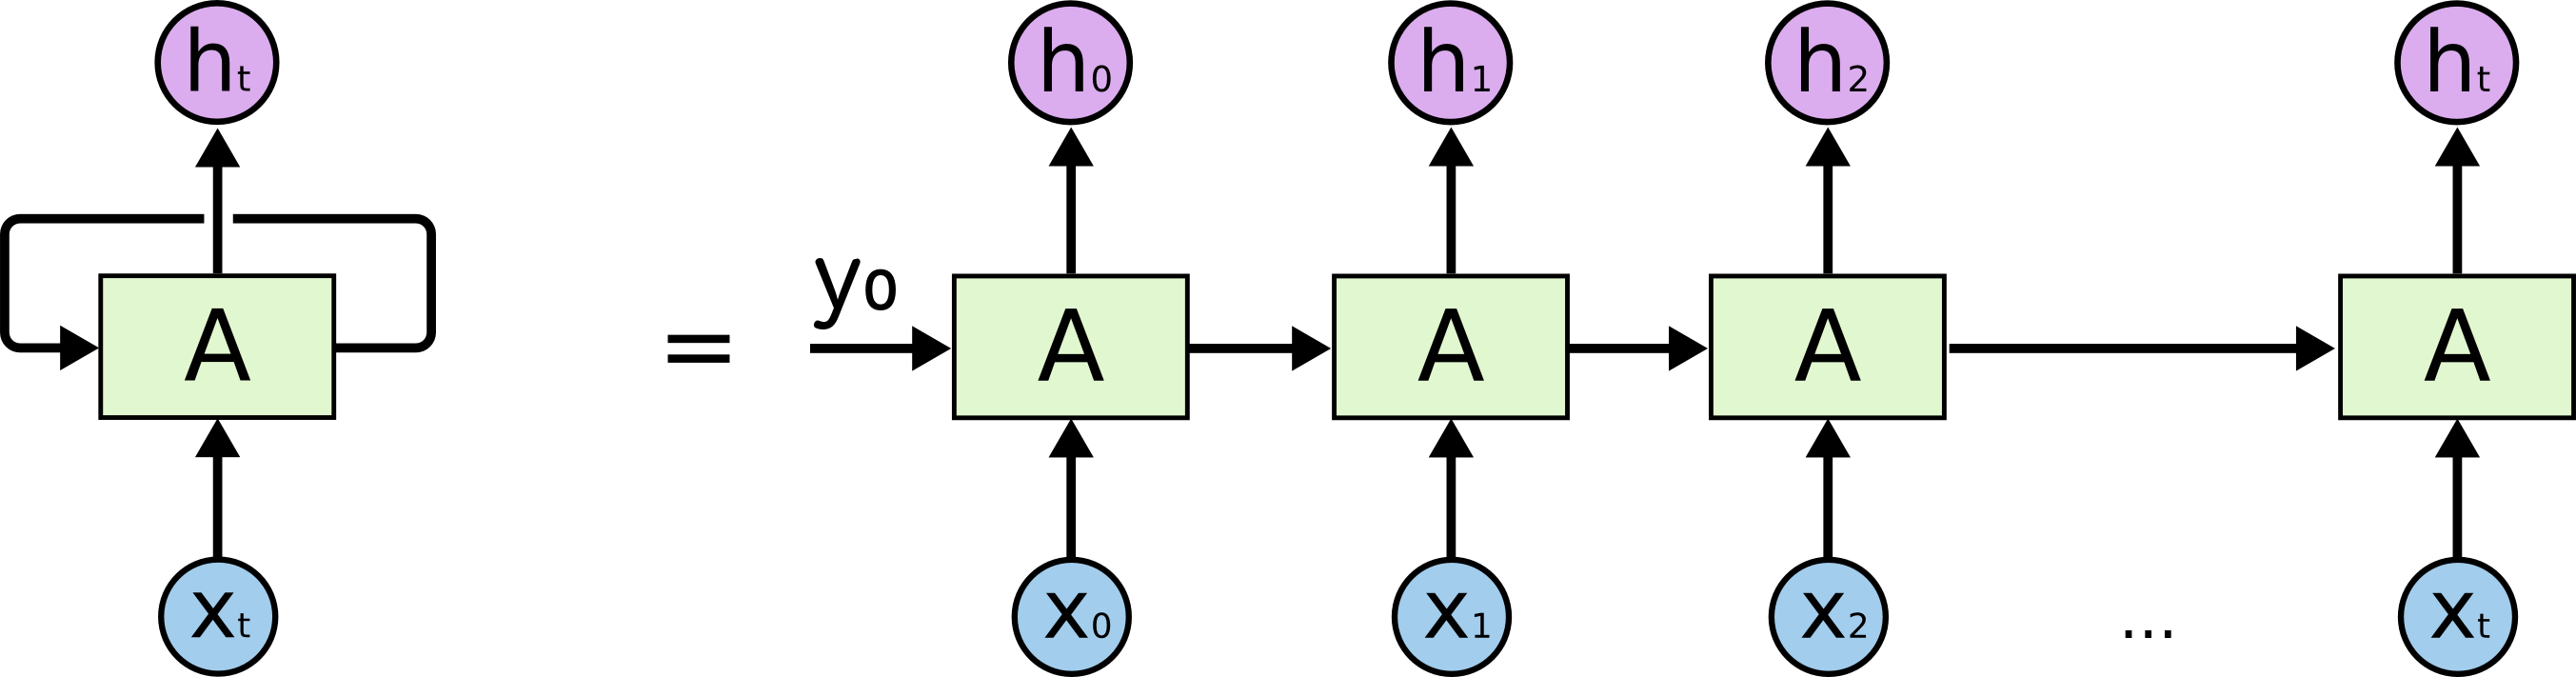
\includegraphics[width=\textwidth]{./img/RNN-unrolled}
  \caption{An unrolled recurrent neural network (taken from \cite{olah:lstm:2015}).}
  \label{fig:RNN-unrolled}
\end{center}
\end{figure}


\subsubsection{Vanishing gradient problem}

During training with backpropagation recurrent neural networks often suffer of the problem of vanishing gradients.
When using BPTT for training a RNN the error gets backpropagated through potentially a great number of layers. The magnitude
of the gradients of $E$ is affected by the weights and the derivatives of the activation function. If either of these amounts
to a factor of $< 1$ then the gradients can vanish over time, because we calculate the gradients with the
chain rule $(f\circ g)'=(f'\circ g)\cdot g'$.
This is a problem with a lot of common activation functions. For example the derivative 
of $\tanh(x)$ will be $< 1$ for all inputs $\neq 0$, 
the derivative of the sigmoid function is always $\frac{\partial sig(x)}{\partial x} \leq 0.25$. 
If a network has a lot of layers a lot of these small numbers get multiplied to calculate their gradient, and subsequently 
these layers train very slowly.
If the gradients can become larger than $1$ the gradients might become very big (exploding gradient problem).

There are a couple of solutions for this problem: With faster hardware the slow training of some layers may not be such a big issue anymore.
Another solution is to avoid recurrent connections with gradients $\neq 1$. This way there are not many factors where the
gradient can vanish. One such example is the LSTM network described in section~\ref{subsec:lstm}. 
The activation function in the recurrency of the LSTM is the identity function, with a derivative of $1$. Therefore the problems described 
above don't apply. There are other methods, but these are beyond our scope here.

%There are two factors that affect the magnitude of gradients - the weights and the activation functions (or more precisely, 
% their derivatives) that the gradient passes through.
%If either of these factors is smaller than 1, then the gradients may vanish in time; 
%if larger than 1, then exploding might happen. For example, the tanh derivative is <1 for all inputs except 0; 
% sigmoid is even worse and is always ≤0.25.


\subsection{Long Short-Term Memory}
\label{subsec:lstm}

A special form of RNN which is designed to "remember" inputs over arbitary distances and "forget" them when necessary.
They avoid the vanishing gradient problem are therefore very popular for tasks that involve any kind of classification,
processing or prediction of time-series data. This ability makes them very well suited for tasks like neural language modeling
or speech tagging where gap's between relevant inputs are likely.
A basic LSTM block will have 3 essential gates:

\begin{itemize}
\item Gate \(i_t\) to determine when to learn an input value
\item Gate \(f_t\) to determine if it should continue to remember or forget the currently stored value
\item Gate \(o_t\) to determine wether it should output the value.
\end{itemize}

The figure~\ref{fig:Long_Short_Term_Memory} below shows a simple LSTM gate, with arrows showing the flow of the values.
The gates with $\bigotimes$ calculate component-wise (Hadamard) product of their inputs. The activation function is usually 
the sigmoid function, except for the input/output gates marked with $\int$, which usually use the $\tanh$ function.

\begin{figure}[H]
\begin{center}
  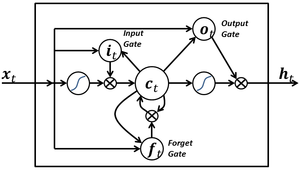
\includegraphics[width=0.7\textwidth]{./img/Long_Short_Term_Memory}
  \caption{A LSTM gate with input, output, and forget gate.}
  \label{fig:Long_Short_Term_Memory}
\end{center}
\end{figure}
Based on the input $x_t$, the remembered value $c_{t-1}$ and the output $h_{t-1}$ the input gates $i_t$, $f_t$ and $o_t$ can
decide how the LSTM behaves. If $i_t$ is close to zero, no input from $x_t$ is stored. If $f_t$ is close to zero,
the LSTM block will forget the stored value. Depending on $o_t$ the block outputs the stored value or not.
The output of $c_t$ is not directly fed through an activation function, so it doesn't automatically decay
over time.
Furthermore there are bias values $b_*$ added to all gates. Bias values can improve the performance of the LSTM compared to other RNN 
architectures according to~\cite{icml2015_jozefowicz15}.

Given the input vectors $x_1,\dots,x_m$ a LSTM computes the output sequence $h_1,\dots, h_{m+1}$ by iteratively applying the
following equations (The $W_*$ variables are the weight matrices of the gates):
\begin{equation}
\begin{aligned}  
  i_t &=\sigma(W_{ix} * x_t  + W_{ih} * h_{t-1} + W_{ic} * c_{t-1} + b_i) \\  
  f_t &=\sigma(W_{fx} * x_t  + W_{fh} * h_{t-1} + W_{fc} * c_{t-1} + b_f) \\
  o_t &=\sigma(W_{ox} * x_t  + W_{oh} * h_{t-1} + W_{oc} * c_t + b_o) \\  
  c_t &= f_t \odot c_{t-1} + i_t \odot \tanh(W_{cx} * x_t  + W_{ch} * h_{t-1} + b_c) \\ 
  h_t &= o_t \odot \tanh(c_t) 
\end{aligned}
\end{equation}

The sigmoid activation function is used for $i_t$, $f_t$, $o_t$ since it's $(0, 1)$ range is suited well for their particular gating decision: 
These gates 'decide' how much of the value to pass through, which is a 0\% to 100\% decision.
The $\tanh$ function is used as the output function, because it saturates at plus / minus one as opposed to zero and one for the sigmoid
function~\cite{Glorot10understandingthe}.

%As we will see, there are more complex variants of the LSTM. For example a possible addition is to feed the output value $h_{t-1}$
%into the gates $i_t$, $f_t$ and $o_t$. This way they can incorporate the actual output into their gating decision.
% It avoids the problem of vanishing gradients, because the gradient of the recurrency function will either be 0 or 1.

\subsection{Unsupervised training: Autoencoder}

An autoencoder transforms an input sequence into a code, and vice versa. 
An autoencoder consists of two parts: the encoder and the decoder. They can be defined as transitions $\phi$ and $\psi$, such that:\\
$\phi:\mathcal{X} \rightarrow \mathcal{F}$\\
$\psi:\mathcal{F} \rightarrow \mathcal{X}$\\
$\arg \min_{\phi,\psi} \|X-(\psi \circ \phi) X\|^2$\\
This will allow us to train a NN to generate word embeddings without the need for labeled data.
Given a sequence of words this NN can learn a mapping where the resulting feature vectors are similar for words which have a similar meaning. 

\begin{figure}[H]
\begin{center}
  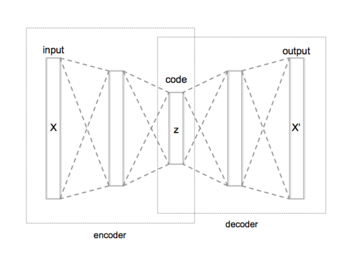
\includegraphics[width=0.5\textwidth]{./img/autoencoder_structure}
  \caption{An autoencoder NN with the encoding and decoding layer}
  \label{fig:autoencoder}
\end{center}
\end{figure}


